\header{
    \headtitle{Les fraises et les framboises} \label{les-fraises-et-les-framboises}
    %
    
    \insertComment{Chanson québéquoise de 1926 de Robert Engel, Serge Goron et Yves Puech.}{}
}

\noindent
\begin{minipage}{0.65\textwidth}
\textbf{Refrain :}
\enluminure{4}{\href{https://www.youtube.com/watch?v=5-soD3qZhy4}{A}}{h ! les fraises} et les framboises
\\Et les vins que nous avons bu
\\Et les belles villageoises
\\Nous ne les r'verons plus
\end{minipage}
\begin{minipage}{0.3\textwidth}
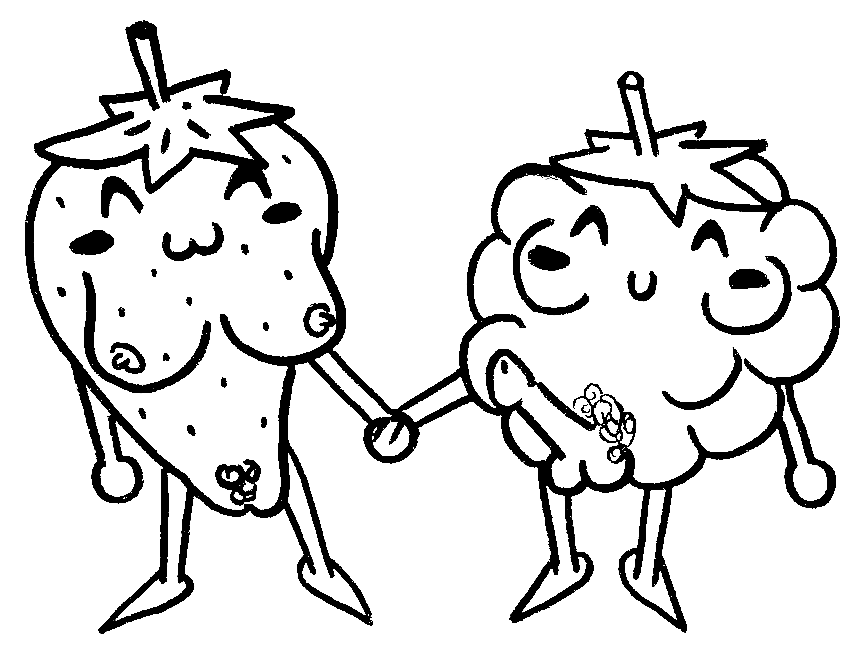
\includegraphics[width=1\textwidth]{images/fraises_framboises.png}
\end{minipage}
\\\\En revenant d'la foire, d'la foire St Michel,
\\J'ai rencontré trois filles, trois filles du pays.
\\\\J'ai rencontré trois filles, trois filles du pays,
\\J'ai choisi la première, la plus jolie aussi.
\\\\J'ai choisi la première, la plus jolie aussi,
\\La monte dans ma chambre, l'allonge sur le lit.
\\\\La monte dans ma chambre, l'allonge sur le lit,
\\J'regarde entre ses jambes, j'aperçois l'Paradis.
\\\\J'regarde entre ses jambes, j'aperçois l'Paradis,
\\J'regarde entre les miennes, j'aperçois Jésus Christ.
\\\\J'regarde entre les miennes, j'aperçois Jésus Christ,
\\Jésus Christ lève la tête et rentre dans l'Paradis.
\\\\Jésus Christ lève la tête et rentre dans l'Paradis,
\\Il s'y fendit le crâne, sa cervelle en jaillit.
\\\\Il s'y fendit le crâne, sa cervelle en jaillit,
\\Pleurez, pleurez, Mesdames, la mort de Jésus Christ.
\\\\Pleurez, pleurez, Mesdames, la mort de Jésus Christ,
\\Mais cinq minutes après, le voilà qui revit.

\breakpage